This document provides an overview of how to prepare documentation for inclusion within {\ttfamily oomph-\/lib}.



 

\hypertarget{index_setup}{}\section{Setting up the documentation}\label{index_setup}
\hypertarget{index_makefiles}{}\subsection{Makefiles}\label{index_makefiles}

\begin{DoxyEnumerate}
\item Within an appropriate subdirectory of the {\ttfamily doc} directory, create a directory for your documentation, e.\+g. 
\begin{DoxyCode}
cd doc/axisym\_navier\_stokes/
mkdir spin\_up
\end{DoxyCode}

\item Add this new directory to the parent directory\textquotesingle{}s {\ttfamily Makefile.\+am} 
\item Add the entry {\ttfamily doc/axisym\+\_\+navier\+\_\+stokes/spin\+\_\+up} to the file {\ttfamily config/configure}. {\ttfamily ac\+\_\+scripts/doc}.{\ttfamily dir\+\_\+list} 
\item Create a new {\ttfamily $\ast$}.{\ttfamily txt} file with the same name as the newly-\/created directory, e.\+g. 
\begin{DoxyCode}
touch spin\_up.txt
\end{DoxyCode}
 This is the \char`\"{}source\char`\"{} file from which the documentation will be generated.
\item From an existing documentation directory, copy across the following files into the newly created directory\+:
\begin{DoxyItemize}
\item {\ttfamily Makefile.\+am} 
\item {\ttfamily Doxyfile} 
\end{DoxyItemize}
\item In {\ttfamily Makefile.\+am} after {\ttfamily \char`\"{}docfile =\char`\"{}}, add the stem of the {\ttfamily $\ast$}.{\ttfamily txt} file created in step 4, e.\+g. 
\begin{DoxyCode}
docfile = spin\_up
\end{DoxyCode}

\item In {\ttfamily Doxyfile} update the (relative) path to the demo-\/driver directory. Two entries must be updated, one following {\ttfamily \char`\"{}\+I\+N\+P\+U\+T\char`\"{}} and the other following {\ttfamily \char`\"{}\+E\+X\+A\+M\+P\+L\+E\+\_\+\+P\+A\+T\+H\char`\"{}}. To find these, search for {\ttfamily \char`\"{}../..\char`\"{}}.
\item Return to {\ttfamily oomph-\/lib\textquotesingle{}s} top-\/level directory and re-\/run {\ttfamily autogen}.{\ttfamily sh\+:} 
\begin{DoxyCode}
./autogen.sh 
\end{DoxyCode}

\end{DoxyEnumerate}\hypertarget{index_figures_setup}{}\subsection{Figures}\label{index_figures_setup}
If your documentation is to contain figures or animations, the following subdirectories must be created within your documentation directory\+:
\begin{DoxyItemize}
\item {\ttfamily figures} 
\begin{DoxyItemize}
\item This must contain all figures used in the documentation in both {\ttfamily $\ast$}.{\ttfamily gif} and {\ttfamily $\ast$}.{\ttfamily eps} formats ({\ttfamily $\ast$}.{\ttfamily gif} is used for the {\ttfamily html} documentation whilst {\ttfamily $\ast$}.{\ttfamily eps} is used for {\ttfamily La\+TeX}).
\end{DoxyItemize}
\item {\ttfamily non\+\_\+distfigures} 
\begin{DoxyItemize}
\item This contains any additional files (etc.) used to create or maintain the documentation. It is good practise to always keep any {\ttfamily $\ast$}.{\ttfamily lay} and {\ttfamily $\ast$}.{\ttfamily lpk} files that were used to create figures, along with any macro ({\ttfamily $\ast$}.{\ttfamily mcr}) files.
\end{DoxyItemize}
\end{DoxyItemize}



\hypertarget{index_write}{}\section{Writing the documentation}\label{index_write}
The \char`\"{}source\char`\"{} of the documentation is contained in the {\ttfamily $\ast$}.{\ttfamily txt} file (a mixture of {\ttfamily html/doxygen} markup). The title must follow the tag {\ttfamily \textbackslash{}mainpage} and be all on one line, e.\+g. 
\begin{DoxyCode}
\(\backslash\)mainpage Demo problem: Spin-up of a viscous fluid
\end{DoxyCode}
 The main body of the text just follows as in a {\ttfamily La\+TeX} document, with line spacings indicating paragraph breaks.\hypertarget{index_html}{}\subsection{H\+T\+ML}\label{index_html}
Any standard html tags can be used (for example, {\ttfamily $<$hr$>$} inserts a horizontal line). Hyperlinks are inserted in the following way\+: 
\begin{DoxyCode}
This is illustrated in an <A HREF=\textcolor{stringliteral}{"../figures/my\_movie.avi"}>animation</A>.
\end{DoxyCode}
 Note that the {\ttfamily \char`\"{}..\char`\"{}} is present in the path above because during the build process the documentation is created in subdirectories of the directory in which the source file is located. See the section \hyperlink{index_generate}{Generating the documentation} below for more details.

To link to the documentation of another demo driver, {\ttfamily poisson/one\+\_\+d\+\_\+poisson} for example, hyperlink to the {\ttfamily index.\+html} file within the {\ttfamily html} directory of that demo driver\textquotesingle{}s documentation. Note that because the processed ({\ttfamily html}) version of the documentation you are working on will live in its own {\ttfamily html} subdirectory, it is necessary to go up three directories in order to be in {\ttfamily oomph-\/lib\textquotesingle{}s} {\ttfamily doc} directory. 
\begin{DoxyCode}
...see <A HREF=\textcolor{stringliteral}{"../../../poisson/one\_d\_poisson/html/index.html"}>the
Poisson tutorial</A>.
\end{DoxyCode}
\hypertarget{index_sections}{}\subsection{Sections}\label{index_sections}
Sections are created as follows\+: 
\begin{DoxyCode}
\(\backslash\)section section\_label This is the title of my section
\end{DoxyCode}


Likewise, subsections are created in the following way\+: 
\begin{DoxyCode}
\(\backslash\)subsection subsection\_label This is the title of my subsection
\end{DoxyCode}


Any {\ttfamily La\+TeX} section types can be used in this way. To link to a section within a document, use the syntax {\ttfamily \textbackslash{}ref} {\ttfamily section\+\_\+label}, as in this example\+: 
\begin{DoxyCode}
...can be found in the section \(\backslash\)ref theory below.
\end{DoxyCode}
\hypertarget{index_equations}{}\subsection{Equations}\label{index_equations}
Equations are generated as in {\ttfamily La\+TeX} except {\ttfamily \textbackslash{}f} must be added before {\ttfamily \$} or {\ttfamily }\mbox{[}, {\ttfamily }\mbox{]}.
\begin{DoxyItemize}
\item E.\+g. inline maths\+: 
\begin{DoxyCode}
...is given by \(\backslash\)f$ \(\backslash\)sin(x) \(\backslash\)f$
\end{DoxyCode}

\item E.\+g. equation environment\+: 
\begin{DoxyCode}
\(\backslash\)f[
\(\backslash\)sin(x)
\(\backslash\)f]
\end{DoxyCode}

\end{DoxyItemize}

To label equations, the normal {\ttfamily La\+TeX} system cannot be used. Instead, mark an equation with the tag {\ttfamily @E{\ttfamily }\mbox{[}L\+A\+B\+EL{\ttfamily }\mbox{]}@} and refer to it later using {\ttfamily @R{\ttfamily }\mbox{[}L\+A\+B\+EL{\ttfamily }\mbox{]}@}, e.\+g.

 
\begin{DoxyImageNoCaption}
  \mbox{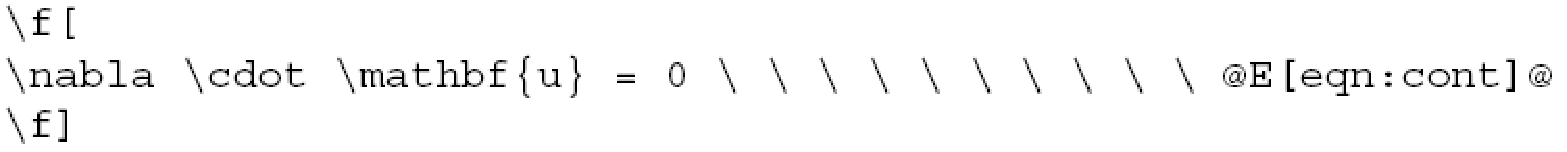
\includegraphics[width=0.71\textwidth]{labelling_example}}
\end{DoxyImageNoCaption}


and then later on... 
\begin{DoxyCode}
...is given by equation (@R[eqn:cont]@).
\end{DoxyCode}
\hypertarget{index_lists}{}\subsection{Lists}\label{index_lists}
To create bullet point lists, precede each item with a {\ttfamily -\/}, e.\+g. 
\begin{DoxyCode}
- First item
- Second item
\end{DoxyCode}
 To create enumerated lists, precede each item with a {\ttfamily -\/\#}, e.\+g. 
\begin{DoxyCode}
-# First item
-# Second item
\end{DoxyCode}
\hypertarget{index_figures}{}\subsection{Figures}\label{index_figures}
A figure with the filename {\ttfamily my\+\_\+figure}.{\ttfamily $\ast$} is inserted in the following way\+:

 
\begin{DoxyImageNoCaption}
  \mbox{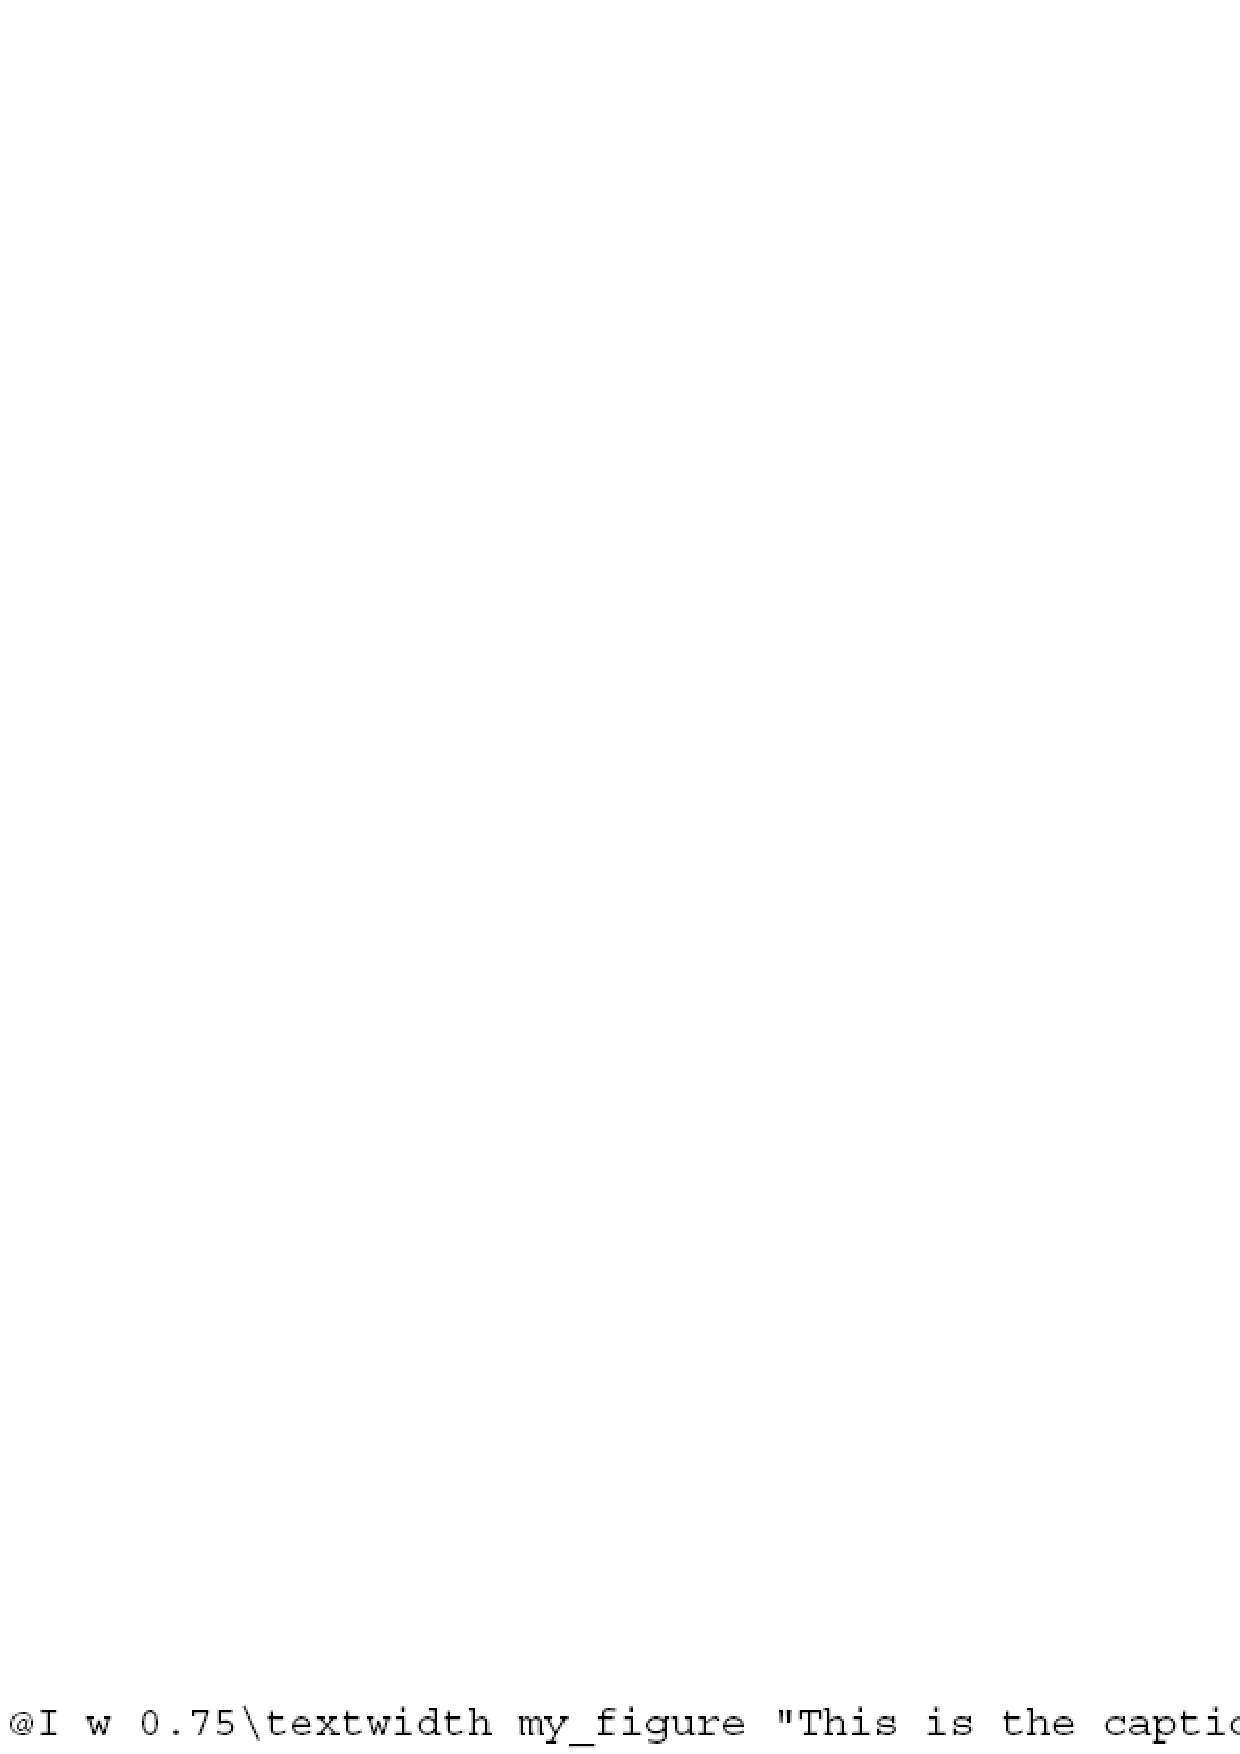
\includegraphics[width=0.71\textwidth]{insert_figures}}
\end{DoxyImageNoCaption}


Note the space between the last character in the caption and the quotation marks. Like the equation labelling, this line is processed by the {\ttfamily txt2h.\+sh} script (which is run automatically as part of the {\ttfamily make} process) and replaced with the necessary commands that tell {\ttfamily doxygen} to use the {\ttfamily $\ast$}.{\ttfamily gif} files for the html documentation and the {\ttfamily $\ast$}.{\ttfamily eps} files for the {\ttfamily La\+TeX} documentation.\hypertarget{index_code}{}\subsection{Code}\label{index_code}
To insert single words of code into prose, precede the word with a {\ttfamily \textbackslash{}c}, e.\+g. 
\begin{DoxyCode}
The function \(\backslash\)c FiniteElement::output(...) is used to...
\end{DoxyCode}


To include blocks of code such as the one immediately above this line of text, use the {\ttfamily \textbackslash{}code} environment, e.\+g.

 
\begin{DoxyImageNoCaption}
  \mbox{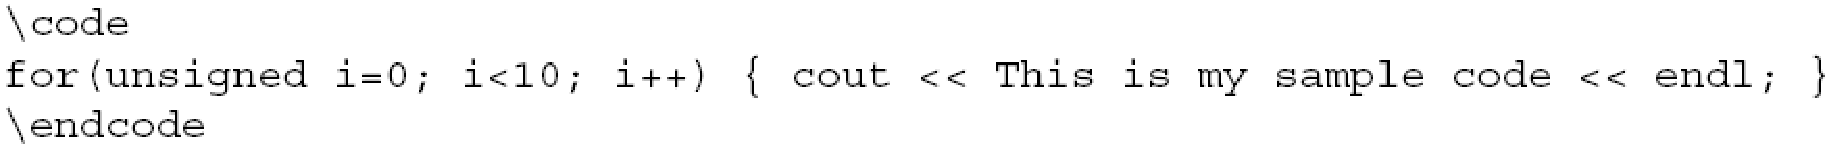
\includegraphics[width=0.71\textwidth]{code_environment}}
\end{DoxyImageNoCaption}


To include sections of the demo code which you are documenting, e.\+g. the main function of {\ttfamily spin\+\_\+up}.{\ttfamily cc}, use the following syntax\+: 
\begin{DoxyCode}
\(\backslash\)dontinclude spin\_up.cc
\(\backslash\)skipline start\_of\_main
\(\backslash\)until end of main
\end{DoxyCode}
 This only works if {\ttfamily start\+\_\+of\+\_\+main} exists somewhere in {\ttfamily spin\+\_\+up}.{\ttfamily cc} file, but any word(s) can be used as a start/endpoint. However, {\bfseries do not use dashes as targets} because more recent versions of doxygen get very confused by this, so {\bfseries don\textquotesingle{}t} do 
\begin{DoxyCode}
\(\backslash\)skipline ----
\end{DoxyCode}
 say.\hypertarget{index_misc}{}\subsection{Miscellaneous}\label{index_misc}

\begin{DoxyItemize}
\item To tell {\ttfamily doxygen} to ignore everything in the source file below a certain point, denote this point with {\ttfamily @@E\+ND@@}.
\item To tell {\ttfamily doxygen} that a certain section of the source file is only to be included in the {\ttfamily html} version of the documentation and omitted in the {\ttfamily La\+TeX} version, enclose this section within {\ttfamily {\ttfamily \textbackslash{}htmlonly} and} {\ttfamily \textbackslash{}endhtmlonly} tags. C\+A\+R\+E\+F\+UL\+: With recent version of doxygen, this has caused problems with certain commands not being interpreted correctly. Best not to use this... The following item is a work-\/around\+:
\item Add the variable {\ttfamily suppress\+\_\+latex\+\_\+in\+\_\+this\+\_\+directory} to the Makefile.\+am and set it to 1 to bypass the generation of latex-\/based documentation for a specific directory (which may contain difficult to render tables etc. and therefore cause latex to hang...). Here\textquotesingle{}s an example of a Makefile.\+am from the directory {\ttfamily doc/order\+\_\+of\+\_\+action\+\_\+functions}\+: 
\begin{DoxyCodeInclude}
suppress\_latex\_in\_this\_directory=1

include $(top\_srcdir)/config/makefile\_templates/doc

docfile = order\_of\_action\_functions
\end{DoxyCodeInclude}

\item To tell {\ttfamily doxygen} that a certain section of the source file is only to be included in the {\ttfamily La\+TeX} version of the documentation and omitted in the {\ttfamily html} version, enclose this section within {\ttfamily {\ttfamily \textbackslash{}latexonly} and} {\ttfamily \textbackslash{}endlatexonly} tags.
\end{DoxyItemize}

\hypertarget{index_generate}{}\section{Generating the documentation}\label{index_generate}
Once the source file has been written, simply type {\ttfamily make} in the documentation directory to build the {\ttfamily html} and {\ttfamily La\+TeX} versions, e.\+g. 
\begin{DoxyCode}
cd doc/axisym\_navier\_stokes/spin\_up
make
\end{DoxyCode}
 Two subdirectories, {\ttfamily html} and {\ttfamily latex}, are now created containing the two versions of the documentation. A {\ttfamily $\ast$}.{\ttfamily pdf} file of the {\ttfamily La\+TeX} version is also placed in the current directory.



 

 \hypertarget{index_pdf}{}\section{P\+D\+F file}\label{index_pdf}
A \href{../latex/refman.pdf}{\tt pdf version} of this document is available. \end{document}
